\section{Projekt Bazy Danych}
    \subsection{Model bazy danych - relacyjna SQL}
        Baza danych jest relacyjna oraz obsługiwana jest na serwerze SQL.
    \subsection{Opis}

            Kod SQL definiuje strukturę bazy danych dla systemu zarządzania informacjami o piłkarzach.

            \begin{enumerate}
                \item Tworzenie bazy danych:\\
                Kod rozpoczyna od próby usunięcia bazy danych "pilkanozna" (jeśli istnieje) i następnie tworzy nową bazę o tej samej nazwie.
                Następnie wybiera tę nowo utworzoną bazę jako aktywną dla dalszych operacji.
                Definicje tabel:
                \item Określa strukturę różnych tabel:\\
                \begin{itemize}
                    \item Tabela "pilkarz" przechowuje informacje o piłkarzach, takie jak imię, nazwisko, dane osobowe, umiejętności piłkarskie i pochodzenie.
                    \item Tabela "awatar" prawdopodobnie zawiera linki do obrazków reprezentujących piłkarzy.
                    \item Tabela "krajpilkarza" przechowuje informacje o krajach, do których należą piłkarze.
                    \item Tabela "numernakoszulce" odnosi się do numerów na koszulkach piłkarzy.
                    \item Tabela "pozycja" zawiera różne pozycje, na których piłkarze mogą grać.
                \end{itemize}
                             
                \item Wstawianie danych:\\
                Dodaje przykładowe dane do tabeli "pozycja", "numernakoszulce" i "krajpilkarza".
            \end{enumerate}

        \subsubsection{Ustawienie uprawnień dla użytkownika}
        \begin{lstlisting}
CREATE USER 'projekt'@'localhost' IDENTIFIED BY 'Pracownia107!'; 
GRANT ALL PRIVILEGES ON pilkanozna.* TO 'projekt'@'localhost';
        \end{lstlisting}

    \pagebreak
    \subsection{Rysunek}
        \begin{figure}[!htb]
            \centering
            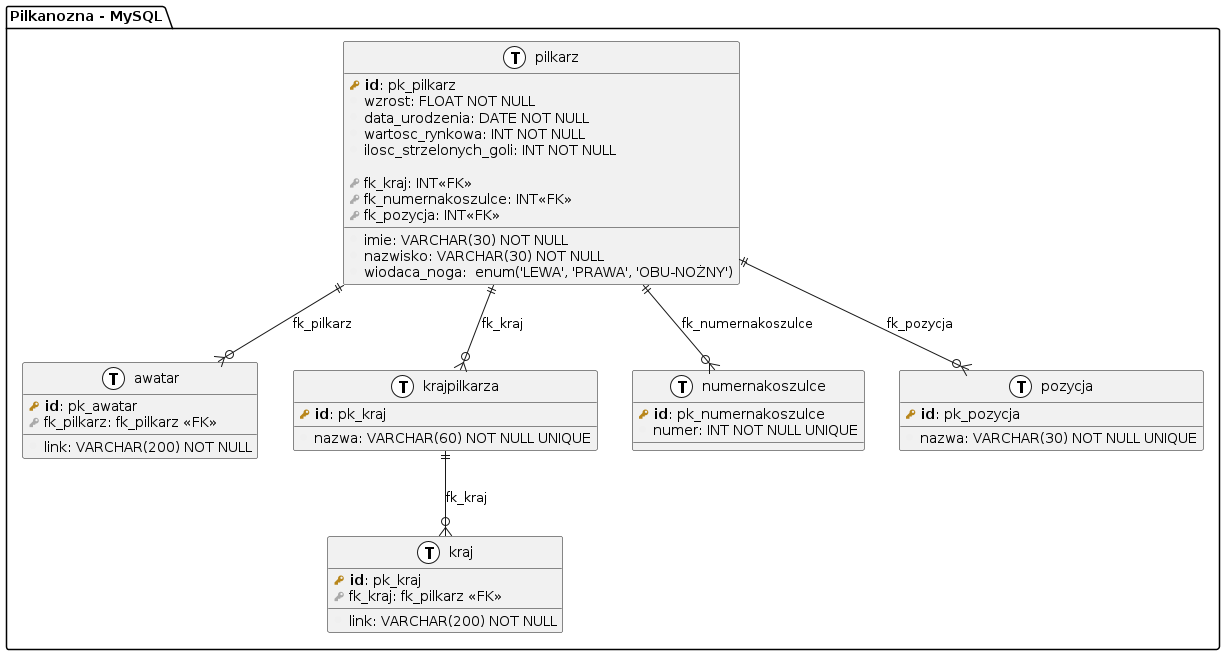
\includegraphics[width=0.9\textwidth]{diagramy/bazy.png}
            \caption{Diagram tabel bazy danych pilkanozna}
        \end{figure}